\documentclass{article}

\usepackage[a4paper, bottom=0.5in, top=0.5in, left=0.5in, right=0.5in]{geometry}
\usepackage{wrapfig}
\usepackage{natbib}
\usepackage{url}
\usepackage{xcolor}
\usepackage{caption}
\usepackage{hyperref}
\hypersetup{
    colorlinks=true,    
    urlcolor=cyan,
}
\usepackage{bytefield}

\usepackage{amsfonts}
\usepackage{float}
\usepackage{enumitem}

\usepackage{minted}

\usepackage{xparse} % NewDocumentCommand, IfValueTF, IFBooleanTF
\usepackage{tikz-timing}[2014/10/29]
\NewDocumentCommand{\busref}{som}{\texttt{%
		#3%
		\IfValueTF{#2}{[#2]}{}%
		\IfBooleanTF{#1}{\#}{}%
}}


\newcommand{\bitFormat}[1]{\emph{\textbf{\textcolor{cyan}{#1}}}}

\newcommand{\regFormat}[1]{\textbf{\textcolor{magenta}{#1}}}

\newcommand{\pinFormat}[1]{\emph{\textcolor{red}{#1}}}


\usepackage{graphicx}
\graphicspath{ {./Resources/pics/} }



\title{ATmega328P Timer/Counter 1}
\author{Narendiran S}
\date{\today}

\begin{document}
\maketitle

\section{Features}
\begin{itemize}
    \item General purpose 8-bit Timer/Counter module.
    \item Two independent output compare units.
    \item Variable PWM.
    \item Three independent interrupt sources (TOV0, OCF0A, and OCF0B).
    \item Clear timer on compare match (auto reload)
\end{itemize}

\section{Block Diagram}
\begin{figure}[H]
    \begin{center}
        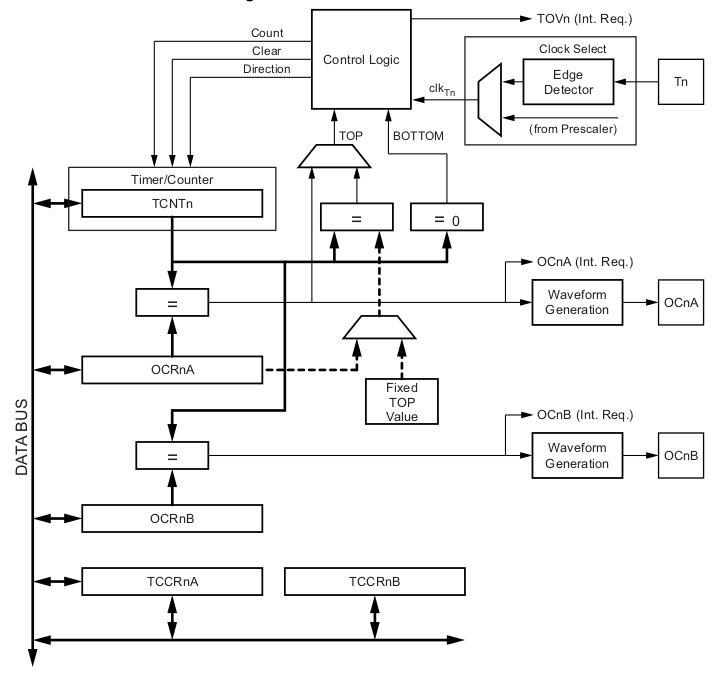
\includegraphics[height=0.6\textheight]{Timer0BlockDiagram.png}
    \end{center}
\end{figure}

\section{Terminologies and Registers}
\begin{minipage}{0.45\textwidth}
    \begin{tabular}{c|p{5.5cm}}
        \textbf{Parameter} & \textbf{Description}\\
        \hline
        BOTTOM & counter reaches 0x00\\
        MAX & ounter reaches 0xFF\\
        TOP & counter reaches highest value (depends on mode of operation can be 0xFF, OCR0A).        
    \end{tabular}
\end{minipage}
\begin{minipage}{0.5\textwidth}
    \begin{tabular}{c|p{6cm}}
        \textbf{Register - 8 bit} & \textbf{Name}\\
        \hline
        \regFormat{TCNT0} & Timer/Counter0 count value\\
        \regFormat{TCCR0A} & Timer/Coutner0 Control Register A\\
        \regFormat{TCCR0B} & Timer/Coutner0 Control Register B\\
        \regFormat{OCBR0A} & Output compare register A\\
        \regFormat{OCBR0B} & Output compare register B\\
        \regFormat{TIFR0} & Timer Interrupt Flag Register\\
        \regFormat{TIMSK0} & Timer interrupt Mask Register\\
    \end{tabular}
\end{minipage}

\section{Timer/Counter0 Units}
\subsection{Clock Source/Select Unit}
\begin{figure}[H]
    \begin{center}
        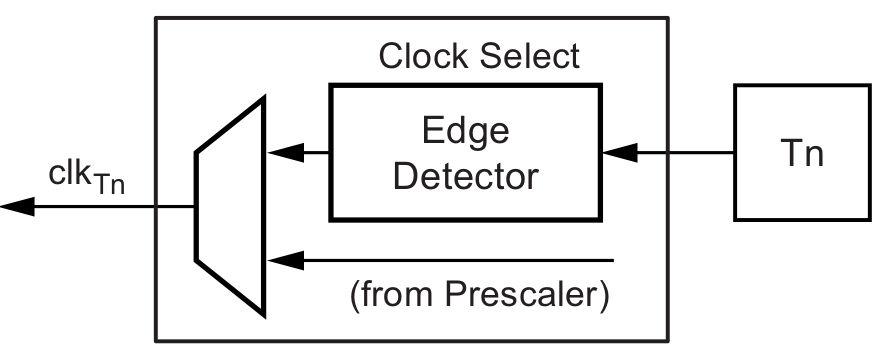
\includegraphics[width=0.5\textwidth]{Timer0ClockSelector.png}
    \end{center}
\end{figure}
\begin{itemize}
    \item The source for the Timer/Counter0 can be external or internal.
    \item External clock source is from \pinFormat{T0} pin.
    \item While Internal Clock source can be clocked via a prescalar.
    \item The output of this unit is the timer clock ($clk_{T0}$).
    \item It uses \bitFormat{CS0[2:0]} bits in \regFormat{TCCR0B} register to select the source.
\end{itemize}


\subsection{Counter Unit}
\begin{minipage}{0.5\textwidth}
    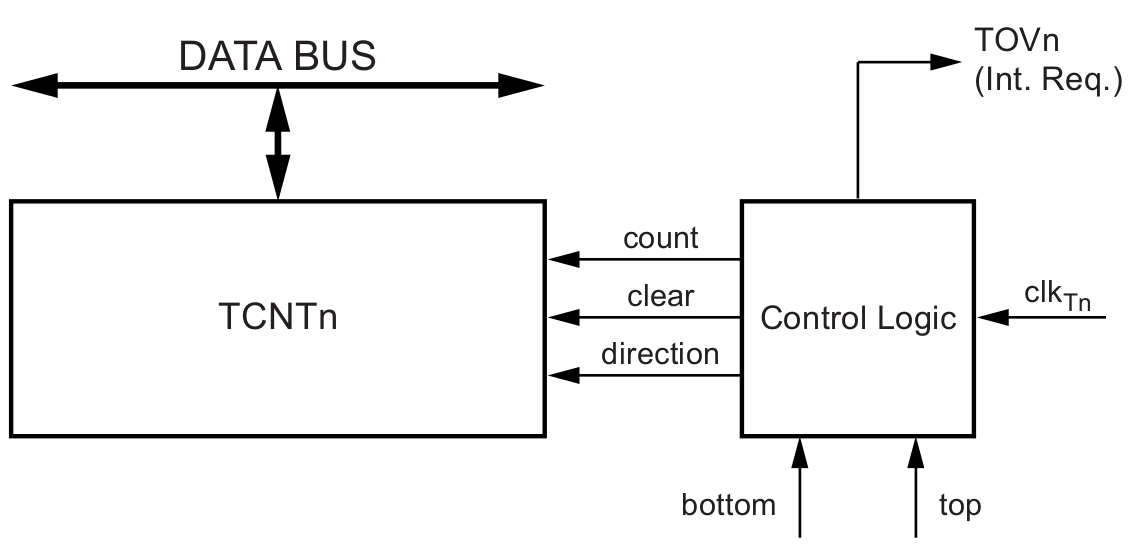
\includegraphics[width=1\textwidth]{Timer0CounterUnit.png}
\end{minipage}
\begin{minipage}{0.45\textwidth}
    \begin{tabular}{c|p{5.5cm}}
        \textbf{Signal} & \textbf{Description}\\
        \hline  
        count & Increment or decrement \regFormat{TCNT0} by 1\\
        direction & Select between increment or decrement\\
        clear & Clears \regFormat{TCNT0} to 0x00\\
        $clk_{T0}$ & Timer/Coutner0 clock\\
        top & Signalize that \regFormat{TCNT0} has maximum value\\
        bottom & Signalize that \regFormat{TCNT0} has minimum value(0x00)\\
    \end{tabular}
\end{minipage}
\begin{itemize}
    \item The main part of the 8-bit Timer/Counter is the programmable bi-directional counter.
    \item Depending the mode of operation the counter is cleared, incremented, or decremented at each timer clock ($clk_{T0}$).
    \item Counting sequence is determined by \bitFormat{WGM0[1:0]} bits of \regFormat{TCCR0A} -Timer/Counter0 Control register A and \bitFormat{WGM02} bit of \regFormat{TCCR0B} - Timer/Counter0 Control register B.
    \item The Timer/Counter0 Overflow flag \bitFormat{TOV0} is set and can generate interrupt according to the mode.
\end{itemize}


\subsection{Output Compare Unit}
\begin{figure}[H]
    \begin{center}
        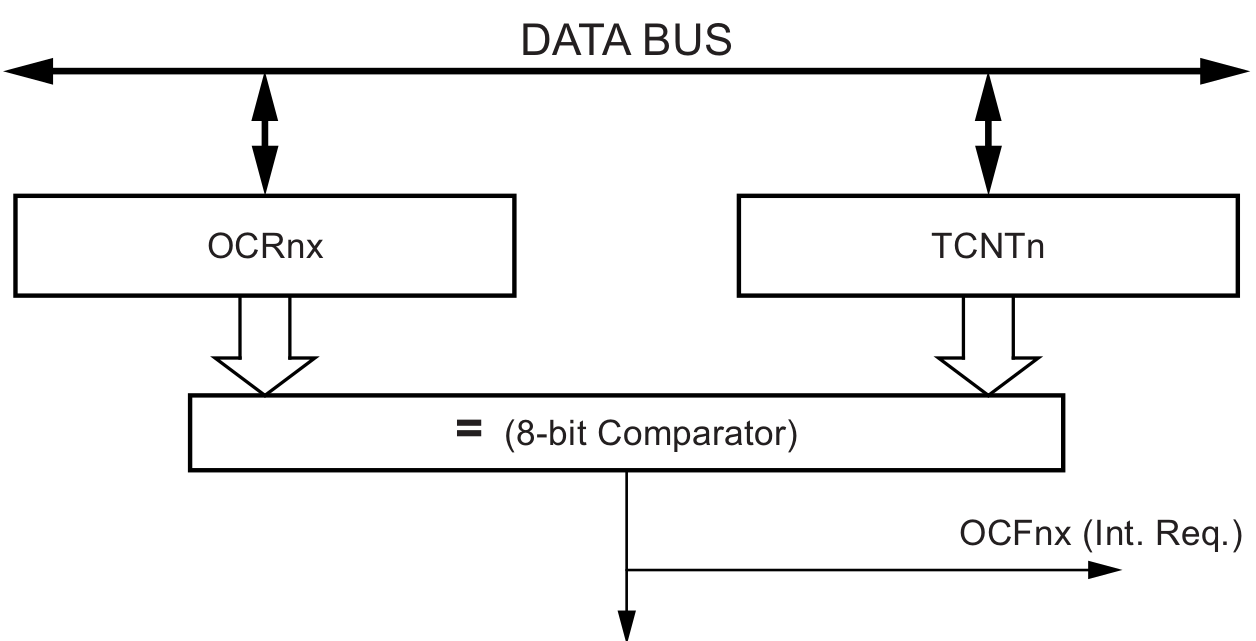
\includegraphics[width=0.5\textwidth]{Timer0CompareUnit.png}
    \end{center}
\end{figure}
\begin{itemize}
    \item 8-bit comparator continuously compares \regFormat{TCNT0} with both \regFormat{OCR0A} and \regFormat{OCR0B}.
    \item When \regFormat{TCNT0} equals \regFormat{OCR0A} or \regFormat{OCR0B}, the comparator signals a match which will set the output compare flag at the next timer clock cycle.
    \item If interrupts are enabled, then output compare interrupt is generated.
    \item The waveform generator uses the match signal to generate an output according to operating mode set by the \bitFormat{WGM0[2:0]} bits and compare output mode \bitFormat{COM0x[1:0]} bits.
\end{itemize}

\subsection{Compare Match Output Unit}
\begin{figure}[H]
    \begin{center}
        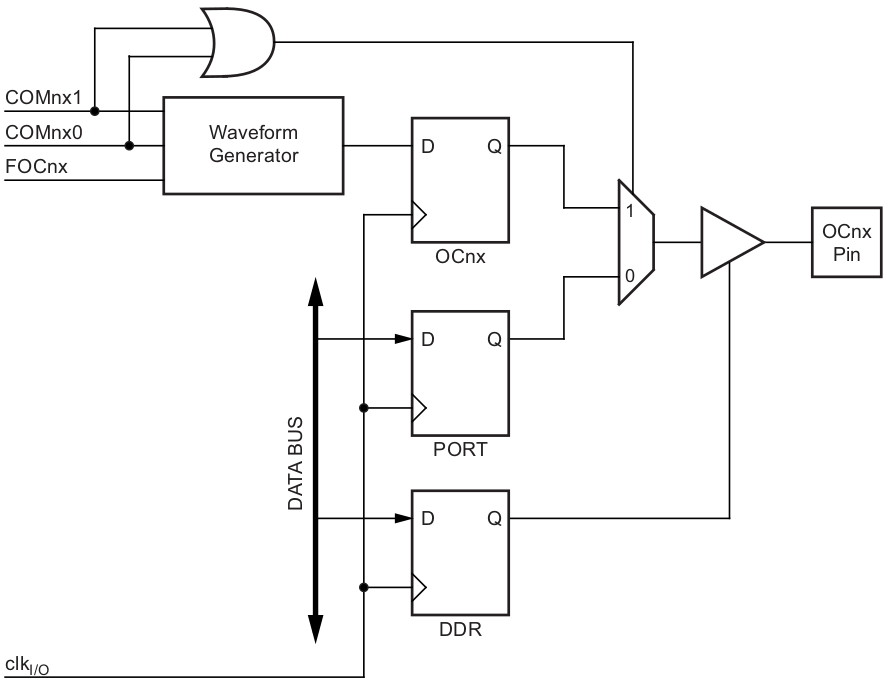
\includegraphics[height=0.3\textheight]{Timer0ComparteMatch.png}
    \end{center}
\end{figure}
\begin{itemize}
    \item This unit is used for changing the state of \pinFormat{OC0A} and \pinFormat{OC0B} pins by configuring the \bitFormat{COM0x[1:0]} bits.
    \item But, general I/O port function is overriiden by DDR reigster.
\end{itemize}

\section{Modes of Operation}
\begin{itemize}
    \item The mode of operation can be defined by combination of waveform generation mode (\bitFormat{WGM0[2:0]}) and compare output mode(\bitFormat{COM0[1:0]}) bits.
    \item The waveform generation mode (\bitFormat{WGM0[2:0]}) bits affect the counting sequence.
    \item For non-PWM mode, \bitFormat{COM0[1:0]} bits control if the output should be set, cleared or toggled at a compare match.
    \item For PWM mode, \bitFormat{COM0[1:0]} bits control if the PWM generated should be inverted or non-inverted.
\end{itemize}

\subsection{Normal Mode - Non-PWM Mode}
\begin{itemize}
    \item \bitFormat{WGM0[2:0]} $-->$ 000.
    \item Counter counts up and no counter clear.
    \item Overruns TOP(0XFF) and restarts from BOTTOM(0X00).
    \item \bitFormat{TOV0} Flag is only set when overrun.
    \item We have to clear \bitFormat{TOV0} flag inorder to have next running.
    \item But, if we use interrupt we don’t need to clear it as interrupt automatically clear the \bitFormat{TOV0} flag.
    \item The timing can be seen below.
\end{itemize}

\begin{tikztimingtable}[
    timing/dslope=0.1,
    timing/.style={x=5ex,y=2ex},
    x=5ex,
    timing/rowdist=3ex,
    timing/name/.style={font=\sffamily\scriptsize}
    ]
    \busref{clk\_{T0}}  & 41{c}\\
    \busref{TCNT0} & u{} D{0x00} D{0x01};[dotted] 2D{};D{0xFE} D{0xFF}D{0x00} D{0x01};[dotted] 2D{};D{0xFE} D{0xFF}D{0x00} D{0x01};[dotted] 2D{};D{0xFE} D{0xFF}D{0x00} D{0x01}\\
    \busref{TOV0} & l 6{L} H 5{L} H 5{L} H 1{L}\\
\end{tikztimingtable}

\subsection{Clear Timer on Compare Match(CTC) Mode - Non-PWM Mode}
\begin{itemize}
    \item \bitFormat{WGM0[2:0]} $-->$ 010.
    \item Counter value clears when \regFormat{TCNT0} reaches \regFormat{OCR0A}.
    \item Interrupt can be generated each time \regFormat{TCNT0} reaches \regFormat{OCR0A} register value by \bitFormat{OCF0A} flag.
    \item When \bitFormat{COM0A[1:0]} == 01, the \pinFormat{OC0A} pin output can be set to toggle its match between \regFormat{TCNT0} and \regFormat{OCR0A} to generate waveform.
    \item The frequency of the waveform its
    \begin{center}
        { \Large $f_{OC0A} = \frac{f_{clkT0}}{2 * N * (1 + OCR0A)}$ }
    \end{center}
    \item Here N is prescalar factor and can be (1, 8, 64, 256, or 1024).
\end{itemize}
\begin{tikztimingtable}[
    timing/dslope=0.1,
    timing/.style={x=5ex,y=2ex},
    x=5ex,
    timing/rowdist=3ex,
    timing/name/.style={font=\sffamily\scriptsize}
    ]
    \busref{clk\_{T0}}  & 28{1.5c}\\
    \busref{TCNT0} & 0.75U{} 1.5D{0x00} 1.5D{0x01};[dotted] 3D{};1.5D{OCR0A - 1} 1.5D{OCR0A}1.5D{0x00} 1.5D{0x01};[dotted] 3D{};1.5D{OCR0A - 1} 1.5D{OCR0A} 1.5D{0x00} 0.75D{0x01} \\
    \busref{OC0A} & 0.75L 9{L} 1.5H l 7{L} 1.5H l\\
\end{tikztimingtable}

\subsection{Fast PWM Mode}
\begin{itemize}
    \item \bitFormat{WGM0[2:0]} $-->$ 011 or 111.
    \item Power Regulation, Rectification, DAC applications.
    \item Single slope operations causing high frequency PWM waveform.
    \item Counter starts from BOTTOM to TOP and then restarts from BOTTOM.
    \item TOP is defined by
    \begin{itemize}
        \item TOP == 0xFF if \bitFormat{WGM0[2:0]} $-->$ 011
        \item TOP == \regFormat{OCR0A} if \bitFormat{WGM0[2:0]} $-->$ 111
    \end{itemize}
    \item  When \bitFormat{COM0A[1:0]} == 01, the \pinFormat{OC0A} pin output can be set to toggle its match between \regFormat{TCNT0} and TOP to generate waveform.
    \begin{itemize}
        \item The above is possible only when \bitFormat{WGM02} bit is set.
        \item And only on \pinFormat{OC0A} pin and not on \pinFormat{OC0B} pin.
    \end{itemize}
    \item In Inverting Compare Mode \bitFormat{COM0A[1:0]} == 10 , the \pinFormat{OC0A} or \pinFormat{OC0B} pins is made 1 on compare match between \regFormat{TCNT0} and TOP and made 0 on reaching BOTTOM.
    \item In Non-Inverting Compare Mode \bitFormat{COM0A[1:0]} == 11 , the \pinFormat{OC0A} or \pinFormat{OC0B} pins is made 0 on compare match between \regFormat{TCNT0} and TOP and 1 made  on reaching BOTTOM.
    \item The Timer/Counter overflow flag (\bitFormat{TOV0}) is set each time the counter reaches TOP.
    \item The PWM frequency is given by 
    \begin{center}
        { \Large $f_{OC0xPWM} = \frac{f_{clkT0}}{N * 256}$ }
    \end{center}
\end{itemize}

\subsubsection{WGM[2:0] == 011}
\begin{tikztimingtable}[
    timing/dslope=0.1,
    timing/.style={x=5ex,y=2ex},
    x=5ex,
    timing/rowdist=3ex,
    timing/name/.style={font=\sffamily\scriptsize}
    ]
    \busref{clk\_{T0}}  & 41{1c} c\\
    \busref{TCNT0} & 0.5U{} D{0x00} 1D{0x01};[dotted] 1.5D{};1D{0xFE} 1D{0xFF}1D{0x00} 1D{0x01};[dotted] 1D{};1D{0xFE} 1D{0xFF} 1D{0x00} 1D{0x01} [dotted] 1D{};1D{0xFE} 1D{0xFF} 1D{0x00} 1D{0x01};[dotted] 1D{};1D{0xFE} 1D{0xFF};\\
    \busref{TOV0} & 6{L} H 4{L} H 4{L} H 4{L} \\
\end{tikztimingtable}

\subsubsection{WGM[2:0] == 011}
\begin{tikztimingtable}[
    timing/dslope=0.1,
    timing/.style={x=5ex,y=2ex},
    x=5ex,
    timing/rowdist=3ex,
    timing/name/.style={font=\sffamily\scriptsize}
    ]
    \busref{clk\_{T0}}  & 41{1c} c\\
    \busref{TCNT0} & 0.5U{} D{0x00} 1D{0x01};[dotted] 1.5D{};1D{\tiny OCR0A -1} 1D{\tiny OCR0A}1D{0x00} 1D{0x01};[dotted] 1D{};1D{\tiny OCR0A -1} 1D{\tiny OCR0A} 1D{0x00} 1D{0x01} [dotted] 1D{};1D{\tiny OCR0A -1} 1D{\tiny OCR0A} 1D{0x00} 1D{0x01};[dotted] 1D{};1D{\tiny OCR0A -1} 1D{\tiny OCR0A};\\
    \busref{TOV0} & 6{L} H 4{L} H 4{L} H 4{L} \\
\end{tikztimingtable}


\subsection{Phase Correct PWM Mode}
\begin{itemize}
    \item \bitFormat{WGM0[2:0]} $-->$ 001 or 101.
    \item High resolution phase correct PWM.
    \item Motor control due to symmetric features
    \item Dual slope operations causing ower frequency PWM waveform.
    \item Counter starts from BOTTOM to TOP and then from TOP to BOTTOM.
    \item TOP is defined by
    \begin{itemize}
        \item TOP == 0xFF if \bitFormat{WGM0[2:0]} $-->$ 001
        \item TOP == \regFormat{OCR0A} if \bitFormat{WGM0[2:0]} $-->$ 101
    \end{itemize}
    \item  When \bitFormat{COM0A[1:0]} == 01, the \pinFormat{OC0A} pin output can be set to toggle its match between \regFormat{TCNT0} and TOP to generate waveform.
    \begin{itemize}
        \item The above is possible only when \bitFormat{WGM02} bit is set.
        \item And only on \pinFormat{OC0A} pin and not on \pinFormat{OC0B} pin.
    \end{itemize}
    \item In Inverting Compare Mode \bitFormat{COM0A[1:0]} == 10 , the \pinFormat{OC0A} or \pinFormat{OC0B} pins is made 1 on compare match between \regFormat{TCNT0} and TOP and made 0 on reaching BOTTOM.
    \item In Non-Inverting Compare Mode \bitFormat{COM0A[1:0]} == 11 , the \pinFormat{OC0A} or \pinFormat{OC0B} pins is made 0 on compare match between \regFormat{TCNT0} and TOP and 1 made  on reaching BOTTOM.
    \item The Timer/Counter overflow flag (\bitFormat{TOV0}) is set each time the counter reaches BOTTOM..
    \item The PWM frequency is given by 
    \begin{center}
        { \Large $f_{OC0xPWM} = \frac{f_{clkT0}}{N * 510}$ }
    \end{center}
\end{itemize}

\subsubsection{WGM[2:0] == 001}
\begin{tikztimingtable}[
    timing/dslope=0.1,
    timing/.style={x=5ex,y=2ex},
    x=5ex,
    timing/rowdist=3ex,
    timing/name/.style={font=\sffamily\scriptsize}
    ]
    \busref{clk\_{T0}}  & 41{1c}\\
    \busref{TCNT0} & 0.5U{} D{0x00} 1D{0x01};[dotted] 1.5D{};1D{0xFE} 1D{0xFF}1D{0xFE} 1D{0xFD};[dotted] 1D{};1D{0x01} 1D{0x00} 1D{0x01}[dotted] 1D{};1D{0xFE} 1D{0xFF} 1D{0xFE} 1D{0xFD};[dotted] 1D{};1D{0x01} 1D{0x00} 1d{0x01};\\
    \busref{TOV0} & l H l 8{L} H 8{L} H l\\
\end{tikztimingtable}

\subsubsection{WGM[2:0] == 101}
\begin{tikztimingtable}[
    timing/dslope=0.1,
    timing/.style={x=5ex,y=2ex},
    x=5ex,
    timing/rowdist=3ex,
    timing/name/.style={font=\sffamily\scriptsize}
    ]
    \busref{clk\_{T0}}  & 41{1c}\\
    \busref{TCNT0} & 0.5U{} D{0x00} 1D{0x01};[dotted] 1.5D{};1D{\tiny OCR0A - 1} 1D{\tiny OCR0A}1D{\tiny OCR0A-1} 1D{\tiny OCR0A-2};[dotted] 1D{};1D{0x01} 1D{0x00} 1D{0x01}[dotted] 1D{};1D{\tiny OCR0A-1} 1D{\tiny OCR0A} 1D{\tiny OCR0A-1} 1D{\tiny OCR0A-2};[dotted] 1D{};1D{0x01} 1D{0x00} 1d{0x01};\\
    \busref{TOV0} & l H l 8{L} H 8{L} H l\\
\end{tikztimingtable}
\newpage
\section{Register Description}
\subsubsection*{TCCR0A – Timer/Counter Control Register A}
\vspace*{0.5cm}
\begin{bytefield}[bitformatting={\large\bfseries},
    endianness=big,bitwidth=0.125\linewidth]{8}
    \bitheader[lsb=0]{0-7} \\
    \bitbox{1}{\small COM0A1}
    \bitbox{1}{\small COM0A0}
    \bitbox{1}{\small COM0B1}
    \bitbox{1}{\small COM0B0}
    \bitbox{1}{\small -}
    \bitbox{1}{\small -}
    \bitbox{1}{\small WGM01}
    \bitbox{1}{\small WGM00}\\
\end{bytefield}

\begin{table}[H]
    \begin{center}
        \begin{tabular}{c|p{4cm}|p{5.2cm}|p{5.2cm}}
            \bitFormat{COM0B[1:0]} & \textbf{Non-PWM modes} & \textbf{Fast PWM} & \textbf{Phase Corrected PWM}\\
            \hline
            00 & No output @ \pinFormat{PD5 - OC0B} pin &  No output @ \pinFormat{PD5 - OC0B} & No output @ \pinFormat{PD5 - OC0B}\\
            \hline
            01 & Toggle \pinFormat{PD5 - OC0B} pin on compare Match. & Reserved & Reserved\\
            \hline
            10 & Clear \pinFormat{PD5 - OC0B} pin on compare Match. & Clear \pinFormat{PD5 - OC0B} on compare match and  set \pinFormat{PD5 - OC0B} at BOTTOM & Clear \pinFormat{PD5 - OC0B} on compare match when up-counting and set \pinFormat{PD5 - OC0B} on compare match when down-counting.\\
            \hline
            11 & Set \pinFormat{PD5 - OC0B} pin on compare Match. & Set \pinFormat{PD5 - OC0B} on compare match and clear \pinFormat{PD5 - OC0B} at BOTTOM & Set \pinFormat{PD5 - OC0B} on compare match when up-counting and clear \pinFormat{PD5 - OC0B} on compare match when down-counting\\
        \end{tabular}
    \end{center}
\end{table}

\begin{table}[H]
    \begin{center}
        \begin{tabular}{c|p{4cm}|p{5.2cm}|p{5.2cm}}
            \bitFormat{COM0A[1:0]} & \textbf{Non-PWM modes} & \textbf{Fast PWM} & \textbf{Phase Corrected PWM}\\
            \hline
            00 & No output @ \pinFormat{PD6 - OC0A} pin &  No output @ \pinFormat{PD6 - OC0A} & No output @ \pinFormat{PD6 - OC0A}\\
            \hline
            01 & Toggle \pinFormat{PD6 - OC0A} pin on compare Match. & When WGM0[2] == 1, Toggle \pinFormat{PD6 - OC0A}  pin on Compare match & Toggle \pinFormat{PD6 - OC0A}  pin on Compare match\\
            \hline
            10 & Clear \pinFormat{PD6 - OC0A} pin on compare Match. & Clear \pinFormat{PD6 - OC0A} on compare match and  set \pinFormat{PD6 - OC0A} at BOTTOM & Clear \pinFormat{PD6 - OC0A} on compare match when up-counting and set \pinFormat{PD6 - OC0A} on compare match when down-counting.\\
            \hline
            11 & Set \pinFormat{PD6 - OC0A} pin on compare Match. & Set \pinFormat{PD6 - OC0A} on compare match and  clear \pinFormat{PD6 - OC0A} at BOTTOM & Set \pinFormat{PD6 - OC0A} on compare match when up-counting and clear \pinFormat{PD6 - OC0A} on compare match when down-counting\\
        \end{tabular}
    \end{center}
\end{table}

\begin{table}[H]
    \begin{center}
        \begin{tabular}{c|c|c|c}
            \bitFormat{WGM0[2:0]} & \textbf{Mode of operation} & \textbf{TOP} & \textbf{TOV0 Flag set on}\\
            \hline
            000 & Normal & 0xFF & MAX\\
            001 & PWM Phase Corrected & 0xFF & BOTTOM\\
            010 & CTC & OCRA & MAX\\
            011 & Fast PWM & 0xFF & MAX\\
            101 & PWM Phase Corrected & OCR0A  & BOTTOM\\
            111 & Fast PWM & OCR0A & TOP\\
        \end{tabular}
    \end{center}
\end{table}

\subsubsection*{TCCR0B – Timer/Counter Control Register B}
\vspace*{0.5cm}
\begin{bytefield}[bitformatting={\large\bfseries},
    endianness=big,bitwidth=0.125\linewidth]{8}
    \bitheader[lsb=0]{0-7} \\
    \bitbox{1}{\small FOC0A}
    \bitbox{1}{\small FOC0B}
    \bitbox{1}{\small -}
    \bitbox{1}{\small -}
    \bitbox{1}{\small WGM02}
    \bitbox{1}{\small CS02}
    \bitbox{1}{\small CS01}
    \bitbox{1}{\small CS00}\\
\end{bytefield}

\begin{table}[H]
    \begin{center}
        \begin{tabular}{c|c}
            \bitFormat{CS0[2:0]} & \textbf{Description(Prescalar)}\\
            \hline
            000 & No clock source(Timer/Counter Stopped)\\
            001 & $clk_{I/O}$ – no prescaling\\
            010 & $\frac{clk_{I/O}}{8}$\\
            011 & $\frac{clk_{I/O}}{64}$\\\
            100 & $\frac{clk_{I/O}}{256}$\\\
            101 & $\frac{clk_{I/O}}{1024}$\\\
            110 & External clock source on \pinFormat{T0} pin. Clock on falling edge.\\
            111 & External clock source on \pinFormat{T0} pin. Clock on rising edge.\\
        \end{tabular}
    \end{center}
\end{table}

\subsubsection*{TIMSK0 – Timer/Counter Interrupt Mask Register}
\vspace*{0.5cm}
\begin{bytefield}[bitformatting={\large\bfseries},
    endianness=big,bitwidth=0.125\linewidth]{8}
    \bitheader[lsb=0]{0-7} \\
    \bitbox{1}{\small -}
    \bitbox{1}{\small -}
    \bitbox{1}{\small -}
    \bitbox{1}{\small -}
    \bitbox{1}{\small -}
    \bitbox{1}{\small OCIE0B}
    \bitbox{1}{\small OCIE0A}
    \bitbox{1}{\small TOIE0}\\
\end{bytefield}

\quad Enable interrupts for compare match between \regFormat{TCNT0} and \regFormat{OCR0A} or \regFormat{TCNT0} and \regFormat{OCR0B} or overflow in \regFormat{TCNT}0.

\subsubsection*{TIFR0 – Timer/Counter 0 Interrupt Flag Register}
\vspace*{0.5cm}
\begin{bytefield}[bitformatting={\large\bfseries},
    endianness=big,bitwidth=0.125\linewidth]{8}
    \bitheader[lsb=0]{0-7} \\
    \bitbox{1}{\small -}
    \bitbox{1}{\small -}
    \bitbox{1}{\small -}
    \bitbox{1}{\small -}
    \bitbox{1}{\small -}
    \bitbox{1}{\small OCIE0B}
    \bitbox{1}{\small OCIE0A}
    \bitbox{1}{\small TOIE0}\\
\end{bytefield}

\quad FLag registers for interrupts on compare match between \regFormat{TCNT0} and \regFormat{OCR0A} or \regFormat{TCNT0} and \regFormat{OCR0B} or overflow in \regFormat{TCNT0}.
\newpage


\section{Configuring the Timer/Counter}
\subsection{Normal Mode}
\subsubsection{As Timer}
\begin{center}
    $ON\_TIME = \frac{max\_count}{\frac{F\_CPU}{PRESCALAR}}$
\end{center}
\begin{itemize}
    \item Depending on PRESCALR value, we get different ON\_TIME.
    \item First, \bitFormat{WGM0[2:0]} bits are configured as 000 for Normal Mode in \regFormat{TCCR0A} and \regFormat{TCCR0B} registers.
    \item Next, \bitFormat{COM0A[1:0]} and/or \bitFormat{COM0A[1:0]} bits are configured to make outputs \pinFormat{OC0A} and/or \pinFormat{OC0B} pins to do nothing, set, clear or toggle in \regFormat{TCCR0A} register.
    \item Next, Interrupt is Enabled by \bitFormat{TOIE0} (overflow enable) in \regFormat{TIMSK0} reigster.
    \item Finally, Timer is started by setting prescalar in \bitFormat{CS0[2:0]} bits as needed prescalar of \regFormat{TCR0B} reigster.
    \item Global Interrupt is enabled.
    \item A interrupt Service Routine for Timer0 overflow is Written.
    \item No need to clear the overflow flag as it is done by hardware.
    \item The timing when both pins \pinFormat{OC0A} and \pinFormat{OC0B} are made to toggle.
\end{itemize}

\begin{tikztimingtable}[
    timing/dslope=0.1,
    timing/.style={x=5ex,y=2ex},
    x=5ex,
    timing/rowdist=3ex,
    timing/name/.style={font=\sffamily\scriptsize}
    ]
    \busref{clk\_{T0}}  & 41{c}\\
    \busref{TCNT0} & u{} D{0x00} D{0x01};[dotted] 2D{};D{0xFE} D{0xFF}D{0x00} D{0x01};[dotted] 2D{};D{0xFE} D{0xFF}D{0x00} D{0x01};[dotted] 2D{};D{0xFE} D{0xFF}D{0x00} D{0x01}\\
    \busref{TOV0} & u h h 5{L} H 5{L} H 5{L} H 1{L}\\
    \busref{OC0A} & l H 5{H} 6{L} 6{H} 2{L}\\
    \busref{OC0B} & h L 5{L} 6{H} 6{L} 2{H}\\
\end{tikztimingtable}
\begin{itemize}
    \item The code can be seen below,
\end{itemize}
\begin{minted}[breaklines,bgcolor=lightgray]{c}
// MOde of operation to Normal Mode -- WGM0[2:0] === 000
// WGM0[2](bit3) from TCCR0B, WGM0[1](bit1)  from TCCR0A, WGM0[0](bit0)  from TCCR0A
TCCR0A = TCCR0A & (~(1<<0) & ~(1<<1));
TCCR0B = TCCR0B & ~(1<<3);

/* What to do when timer reaches the MAX(0xFF) value */	
// toggle OC0A and OC0B on each time when reaches the MAX(0xFF) 
// which is reflected in PD6 and PD5

// Output OC0A to toglle when reaches MAX -- COM0A[1:0] === 01
// COM0A[1](bit7) from TCCR0A, COM0A[0](bit6) from TCCR0A
TCCR0A = TCCR0A & ~(1<<7);
TCCR0A = TCCR0A | (1<<6);

// Output OC0B to toglle when reaches MAX -- COM0B1:0] === 01
// COM0B[1](bit7) from TCCR0A, COM0B[0](bit6) from TCCR0A
TCCR0A = TCCR0A & ~(1<<5);
TCCR0A = TCCR0A | (1<<4);

//Enable Interrupt of OVERFLOW flag so that interrupt can be generated
TIMSK0 = TIMSK0 | (1<<0);	

// start timer by setting the clock prescalar
// DIVIDE BY 8 from I/O clock
// DIVIDE BY 8-- CS0[2:0] === 010
// CS0[2](bit2) from TCCR0B,CS0[1](bit1) from TCCR0B,CS0[0](bit0) from TCCR0B
TCCR0B = TCCR0B | (1<<1);
TCCR0B = TCCR0B & (~(1<<0) & ~(1<<2));

// enabling global interrupt
sei();
// SO ON TIME = max_count / (F_CPU / PRESCALAR)
// ON TIME = 0xFF / (16000000/8) = 128us
// since symmetric as toggling OFF TIME = 128us
// hence, we get a square wave of fequency 1 / 256us = 3.906kHz
\end{minted}

\begin{minted}[breaklines,bgcolor=lightgray]{c}
ISR(TIMER0_OVF_vect)
{
    // do the thing when overflows.
}
\end{minted}


\subsubsection{As Counter}
\begin{itemize}
    \item Every rising/falling edge the count increases.
    \item So to reach 256 count, it would take a time of $\frac{0xFF}{frequency @ \pinFormat{T0} pin}$.
    \item First, \bitFormat{WGM0[2:0]} bits are configured as 000 for Normal Mode in \regFormat{TCCR0A} and \regFormat{TCCR0B} registers.
    \item Finally, Counter is started by configuring \bitFormat{CS0[2:0]} bits to 110 or 111 for external falling or rising edge on \pinFormat{T0 - PD4}.
    \item The code when \pinFormat{T0} pin is used as counter @ falling edge.
\end{itemize}

\begin{minted}[breaklines,bgcolor=lightgray]{c}
// MOde of operation to Normal Mode -- WGM0[2:0] === 000
// WGM0[2](bit3) from TCCR0B, WGM0[1](bit1)  from TCCR0A, WGM0[0](bit0)  from TCCR0A
TCCR0A = TCCR0A & (~(1<<0) & ~(1<<1));
TCCR0B = TCCR0B & ~(1<<3);
    
/* to count external event -we must connect source to T0 (PD4) */
// THE CLK IS CLOCKED FROM external source
// Falling edge of T0(PD4) -- CS0[2:0] === 110
// CS0[2](bit2) from TCCR0B,CS0[1](bit1) from TCCR0B,CS0[0](bit0) from TCCR0B
TCCR0B = TCCR0B | (1<<2);
TCCR0B = TCCR0B | (1<<1);
TCCR0B = TCCR0B & ~(1<<0);	
\end{minted}

\subsubsection{Application I - Delay}
\begin{minted}[breaklines,bgcolor=lightgray]{c}
/* TCNT0 starts from 0X00 goes upto 0XFF and restarts */
/* No possible use case as it just goes upto 0xFF and restarts */
// MOde of operation to Normal Mode -- WGM0[2:0] === 000
// WGM0[2](bit3) from TCCR0B, WGM0[1](bit1)  from TCCR0A, WGM0[0](bit0)  from TCCR0A
TCCR0A = TCCR0A & (~(1<<0) & ~(1<<1));
TCCR0B = TCCR0B & ~(1<<3);

/* What to do when timer reaches the MAX(0xFF) value */
// nothing should be done on OC0A for delay
// nothing  -- COM0A[1:0] === 00
// COM0A[1](bit7) from TCCR0A, COM0A[0](bit6) from TCCR0A
TCCR0A = TCCR0A & ~(1<<7);
TCCR0A = TCCR0A & ~(1<<6);
    
/* The delay possible = 0xff / (F_CPU/prescalar) */
// lowest delay = 0xff / (16000000 / 1) = 16us
// when prescalar == 8 --> delay = 0xff / (16000000 / 8) = 128us
// when prescalar == 64 --> delay = 0xff / (16000000 / 64) = 1.024ms
// when prescalar == 256 --> delay = 0xff / (16000000 / 256) = 4.096ms
// highest delay possible = 0xff / (16000000 / 1024) = 16.38ms

// start timer by setting the clock prescalar
// DIVIDE BY 8 use the same clock from I/O clock
// DIVIDE BY 8-- CS0[2:0] === 010
// CS0[2](bit2) from TCCR0B,CS0[1](bit1) from TCCR0B,CS0[0](bit0) from TCCR0B
TCCR0B = TCCR0B & ~(1<<0);
TCCR0B = TCCR0B | (1<<1);
TCCR0B = TCCR0B & ~(1<<2);


// actual delaying - wait until delay happens
while((TIFR0 & 0x01) == 0x00); // checking overflow flag when overflow happns
// clearing the overflag so that we can further utilize
TIFR0 = TIFR0 | 0x01;
\end{minted}

\subsection{CTC Mode}
\subsubsection{As Timer}

\begin{center}
    $ON\_TIME = \frac{1 + OCR0A}{\frac{F\_CPU}{PRESCALAR}}$
\end{center}
\begin{itemize}
    \item Depending on \regFormat{OCR0A} register and PRESCALR value, we get different ON\_TIME.
    \item First, \bitFormat{WGM0[2:0]} bits are configured as 010 for CTC Mode in \regFormat{TCCR0A} and \regFormat{TCCR0B} registers.
    \item Next, \bitFormat{COM0A[1:0]} and/or \bitFormat{COM0B[1:0]} bits are configured to make outputs \pinFormat{OC0A} and/or \pinFormat{OC0B} pins to do nothing, set, clear or toggle in \regFormat{TCCR0A} register.
    \item Next, Interrupt is Enabled by \bitFormat{OCIE01A} (utput compare on match on \regFormat{OCR0A} register enable) in \regFormat{TIMSK0} reigster.
    \item Finally, Timer is started by setting prescalar in \bitFormat{CS0[2:0]} bits as needed prescalar of \regFormat{TCR0B} reigster.
    \item Global Interrupt is enabled.
    \item A interrupt Service Routine for Timer0 Compare is Written.
    \item No need to clear the overflow flag as it is done by hardware.
    \item The timing when both pins \pinFormat{OC0n} are made to toggle.
\end{itemize}


\begin{tikztimingtable}[
    timing/dslope=0.1,
    timing/.style={x=5ex,y=2ex},
    x=5ex,
    timing/rowdist=3ex,
    timing/name/.style={font=\sffamily\scriptsize}
    ]
    \busref{clk\_{T0}}  & 41{c}\\
    \busref{TCNT0} & u{} D{0x00} D{0x01};[dotted] 2D{};D{\tiny OCR0A - 1} D{\tiny OCR0A}D{0x00} D{0x01};[dotted] 2D{};D{\tiny OCR0A - 1} D{\tiny OCR0A }D{0x00} D{0x01};[dotted] 2D{};D{\tiny OCR0A - 1} D{\tiny OCR0A}D{0x00} D{0x01}\\
    \busref{TOV0} & u h h 5{L} H 5{L} H 5{L} H 1{L}\\
    \busref{OC0A} & l H 5{H} 6{L} 6{H} 2{L}\\
    \busref{OC0B} & h L 5{L} 6{H} 6{L} 2{H}\\
\end{tikztimingtable}
\begin{itemize}
    \item The code can be seen below,
\end{itemize}
\begin{minted}[breaklines,bgcolor=lightgray]{c}
// MOde of operation to CTC Mode -- WGM0[2:0] === 010
// WGM0[2](bit3) from TCCR0B, WGM0[1](bit1)  from TCCR0A, WGM0[0](bit0)  from TCCR0A
TCCR0A = TCCR0A & ~(1<<0);
TCCR0A = TCCR0A | (1<<1);
TCCR0B = TCCR0B & ~(1<<3);

/* What to do when timer reaches the OCR0A */
// toggle OC0A on each time when reaches the OCR0A
// which is reflected in PD6
// Output OC0A to toglle when reaches MAX -- COM0A[1:0] === 01
// COM0A[1](bit7) from TCCR0A, COM0A[0](bit6) from TCCR0A
TCCR0A = TCCR0A & ~(1<<7);
TCCR0A = TCCR0A | (1<<6);

// Output OC0B to toglle when reaches MAX -- COM0B1:0] === 01
// COM0B[1](bit7) from TCCR0A, COM0B[0](bit6) from TCCR0A
TCCR0A = TCCR0A & ~(1<<5);
TCCR0A = TCCR0A | (1<<4);

    
// Enable Interrupt when counter matches OCR0A Rgister
//  OCIE0A bit is enabled
TIMSK0 = TIMSK0 | (1<<1);


// setting the value till the counter should reach in OCR0A
// for toggling of OC0A pin
OCR0A = 0x32;

// start timer by setting the clock prescalar
// DIVIDE BY 8 from I/O clock
// DIVIDE BY 8-- CS0[2:0] === 010
// CS0[2](bit2) from TCCR0B,CS0[1](bit1) from TCCR0B,CS0[0](bit0) from TCCR0B
TCCR0B = TCCR0B | (1<<1);
TCCR0B = TCCR0B & (~(1<<0) & ~(1<<2));

// enabling global interrupt
sei();
// SO ON TIME = (1 + OCR0A) / (F_CPU / PRESCALAR)
// ON TIME = 0X32 / (16000000/8) = 25.5us
// since symmetric as toggling OFF TIME = 25.5us
// hence, we get a square wave of fequency 1 / 50us = 20kHz
\end{minted}

\begin{minted}[breaklines,bgcolor=lightgray]{c}
ISR(TIMER0_COMPA_vect)
{
    // do the thing when compare match between TCNT0 matches OCR0A.
}
\end{minted}


\subsubsection{As Counter}
\begin{itemize}
    \item Every rising/falling edge the count increases.
    \item So to reach required count, it would take a time of $\frac{OCR0A}{frequency @ \pinFormat{T0} pin}$.
    \item First, \bitFormat{WGM0[2:0]} bits are configured as 010 for CTC Mode in \regFormat{TCCR0A} and \regFormat{TCCR0B} registers.
    \item Finally, Counter is started by configuring \bitFormat{CS0[2:0]} bits to 110 or 111 for external falling or rising edge on \pinFormat{T0 - PD4} pin.
    \item The code when \pinFormat{T0} pin is used as counter @ falling edge.
\end{itemize}

\begin{minted}[breaklines,bgcolor=lightgray]{c}
// MOde of operation to CTC Mode -- WGM0[2:0] === 010
// WGM0[2](bit3) from TCCR0B, WGM0[1](bit1)  from TCCR0A, WGM0[0](bit0)  from TCCR0A
TCCR0A = TCCR0A & ~(1<<0);
TCCR0A = TCCR0A | (1<<1);
TCCR0B = TCCR0B & ~(1<<3);
    
// Disbale Interrupt when counter matches OCR0A Rgister
//  OCIE0A bit is disabled
TIMSK0 = TIMSK0 & ~(1<<1);

//we count till OCR0A register value and reset and continue 
OCR0A = 0xA;

/* to count external event -we must connect source to T0 (PD4) */
// THE CLK IS CLOCKED FROM external source
// Falling edge of T0(PD4) -- CS0[2:0] === 110
// CS0[2](bit2) from TCCR0B,CS0[1](bit1) from TCCR0B,CS0[0](bit0) from TCCR0B
TCCR0B = TCCR0B | (1<<2);
TCCR0B = TCCR0B | (1<<1);
TCCR0B = TCCR0B & ~(1<<0);
\end{minted}

\subsubsection{Application I - Delay in ms}

\begin{minted}[bgcolor=lightgray]{c}
// minimum delay being 4us -- choose like that
// use PRESCALAR OF 1 -- 3us - 16us -- usage 3us - 16us -- factor=0 -- CS0[2:0]=1
// use PRESCALAR OF 8 -- 3us - 128us -- usage 17us - 128us -- factor=3 -- CS0[2:0]=2
// use PRESCALAR OF 64 -- 4us - 1.024ms -- usage 129us - 1024us -- factor=6 -- CS0[2:0]=3
// use PRESCALAR OF 256 -- 16us - 4.096ms -- usage 1025us - 4096us -- factor=8 -- CS0[2:0]=4
    
// MOde of operation to ctc Mode -- WGM0[2:0] === 010
// WGM0[2](bit3) from TCCR0B, WGM0[1](bit1)  from TCCR0A, WGM0[0](bit0)  from TCCR0A
TCCR0A = TCCR0A & ~(1<<0);
TCCR0A = TCCR0A | (1<<1);
TCCR0B = TCCR0B & ~(1<<3);

while(delayInMs--)
{
    // for 1ms delay
    OCR0A = 249;
    // start timer by setting the clock prescalar
    //  dived by 64 from I/O clock
    //  CS0[2:0] === 011
    // CS0[2](bit2) from TCCR0B,CS0[1](bit1) from TCCR0B,CS0[0](bit0) from TCCR0B
    TCCR0B = TCCR0B | (1<<0);
    TCCR0B = TCCR0B | (1<<1);
    TCCR0B = TCCR0B & ~(1<<2);

    // actual delaying - wait until delay happens
    while((TIFR0 & 0x02) == 0x00); // checking OCF0A (compare match flag A) flag when match happns
    // clearing the compare match flag so that we can further utilize
    TIFR0 = TIFR0 | 0x02;
}
\end{minted}

\subsection{Fast PWM Mode}
\begin{minted}[bgcolor=lightgray]{c}
ISR(TIMER0_OVF_vect)
{
} 
ISR(TIMER0_COMPA_vect)
{
}
ISR(TIMER0_COMPB_vect)
{
}
\end{minted}
\subsubsection{Non-Inverting  PWM with TOP at MAX(0xFF)}
\quad Frequency is chosen by PRESCALAR and Duty cycle by \regFormat{OCR0A} and/or \regFormat{OCR0B} register.
\begin{itemize}
    \item First, \bitFormat{WGM0[2:0]} bits are configured as 011 for Fast PWM Mode with TOP at MAX in \regFormat{TCCR0A} and \regFormat{TCCR0B} registers.
    \item Next, \bitFormat{COM0A[1:0]} and/or \bitFormat{COM0B[1:0]} bits of \regFormat{TCCR0A} register are configured to make outputs \pinFormat{OC0A} and/or \pinFormat{OC0B} pins to generate PWM by comparing between \regFormat{OCR0A} and/or \regFormat{OCR0B} respectively. That is for Non-Inverting, \bitFormat{COM0x[1:0]} is written 10.
    \item Next, the duty cycle value is loaded into \regFormat{OCR0A} and/or \regFormat{OCR0B} register for \pinFormat{OC0A} and/or \pinFormat{OC0B} pins.
    \item Also, the \bitFormat{OCIE0A} and/or \bitFormat{OCIE0B} bits of \regFormat{TIMSK0} register  are enabled for Output Compare Interupts if needed.
    \item The interrupt Service routine is written if needed for compare match.
    \item Finally, Timer is started by setting \bitFormat{CS0[2:0]} bit as needed prescalar in \regFormat{TCR0B} register.
    \item The timing for PWM on 10\% duty cycle \pinFormat{OC0A} and 75\% duty cycle\pinFormat{OC0B} pins are shown assuming .
    \begin{itemize}
        \item 0x19 for OCR0A.
        \item 0xC0 for OCR0B.
    \end{itemize}
\end{itemize}

\begin{tikztimingtable}[
    timing/dslope=0.1,
    timing/.style={x=5ex,y=2ex},
    x=5ex,
    timing/rowdist=3ex,
    timing/name/.style={font=\sffamily\scriptsize}
    ]
    \busref{clk\_{T0}}  & 41{1c} \\
    \busref{TCNT0} & 0.5U{} D{0x00} 1D{0x01};[dotted] 1.5D{};1D{0x19} 1D{0x1A} [dotted] 1.5D{}; 1D{0xC0} 1D{0xC1} [dotted] 1.5D{};1D{0xFF} 1D{0x00} D{0x01} ;[dotted] 1.5D{};1D{0x19} 1D{0x1A} [dotted] 1.5D{};1D{0xBF} 1d{0xC0}\\
    \busref{OC0A} & u H H H h l L L L L L L L l H H H h L L L L L\\
    \busref{OC0B} & u H H H h HHH h L L L L l H H H h HHH Hhl\\
\end{tikztimingtable}

\begin{minted}[bgcolor=lightgray]{c}
// MOde of operation to fast_pwm_top_max Mode -- WGM0[2:0] === 011
// WGM0[2](bit3) from TCCR0B, WGM0[1](bit1)  from TCCR0A, WGM0[0](bit0)  from TCCR0A
TCCR0A = TCCR0A | (1<<0);
TCCR0A = TCCR0A | (1<<1);
TCCR0B = TCCR0B & ~(1<<3);	

// here we set COM0A[1:0] as 10 for non-inverting
// here we set COM0B[1:0] as 10 for non-inverting

// which is reflected in PD6
// COM0A[1](bit7) from TCCR0A, COM0A[0](bit6) from TCCR0A
TCCR0A = TCCR0A | (1<<7);
TCCR0A = TCCR0A & ~(1<<6);

// which is reflected in PD65
// COM0B[1](bit5) from TCCR0A, COM0B[0](bit4) from TCCR0A
TCCR0A = TCCR0A | (1<<5);
TCCR0A = TCCR0A & ~(1<<4);

// Enable Interrupt when TCN0 overflows TOP - here 0xFF
//  TOV0 bit is enabled
TIMSK0 = TIMSK0 | (1<<0);

/* we use OCF0A flag - which is set at every time TCN0 reaches OCR0A 
here we clear led(PC1),  so that we obtain the PWM when TCN0 reaches OCR0A*/
TIMSK0 = TIMSK0 | (1<<1);
/* we use OCF0B flag - which is set at every time TCN0 reaches OCR0B 
here we clear led(PC2),  so that we obtain the PWM when TCN0 reaches OCR0B*/
TIMSK0 = TIMSK0 | (1<<2);


// Next we set values for OCR0A and OCR0B
// Since, TCNT0 goes till max(0xFF), we can choose OCR0A and OCR0B to any value below max(0xFFF)
OCR0A = 0x19; // for 10% duty clcle
OCR0B = 0xC0; // for 75% duty clcle


// start the timer by selecting the prescalr
//  use the same clock from I/O clock
//  CS0[2:0] === 001
// CS0[2](bit2) from TCCR0B,CS0[1](bit1) from TCCR0B,CS0[0](bit0) from TCCR0B
TCCR0B = TCCR0B | (1<<0);
TCCR0B = TCCR0B & ~(1<<1);
TCCR0B = TCCR0B & ~(1<<2);

//enabled global interrupt
sei();
\end{minted}

\subsubsection{Inverting PWM with TOP at MAX(0xFF)}
\quad Frequency is chosen by PRESCALAR and Duty cycle by \regFormat{OCR0A} and/or \regFormat{OCR0B} register.
\begin{itemize}
    \item First, \bitFormat{WGM0[2:0]} bits are configured as 011 for Fast PWM Mode with TOP at MAX in \regFormat{TCCR0A} and \regFormat{TCCR0B} registers.
    \item Next, \bitFormat{COM0A[1:0]} and/or \bitFormat{COM0B[1:0]} bits of \regFormat{TCCR0A} register are configured to make outputs \pinFormat{OC0A} and/or \pinFormat{OC0B} pins to generate PWM by comparing between \regFormat{OCR0A} and/or \regFormat{OCR0B} respectively. That is for Inverting, \bitFormat{COM0x[1:0]} is written 11.
    \item Next, the duty cycle value is loaded into \regFormat{OCR0A} and/or \regFormat{OCR0B} register for \pinFormat{OC0A} and/or \pinFormat{OC0B} bits.
    \item Also, the \bitFormat{OCIE0A} and/or \bitFormat{OCIE0B} bits of \regFormat{TIMSK0} register  are enabled for Output Compare Interupts if needed.
    \item The interrupt Service routine is written if needed for compare match.
    \item Finally, Timer is started by setting \bitFormat{CS0[2:0]} bit as needed prescalar in \regFormat{TCR0B} register.
    \item The timing for PWM on 10\% duty cycle \pinFormat{OC0A} and 75\% duty cycle \pinFormat{OC0B} pins are shown assuming .
    \begin{itemize}
        \item 0x19 for OCR0A.
        \item 0xC0 for OCR0B.
    \end{itemize}
\end{itemize}

\begin{tikztimingtable}[
    timing/dslope=0.1,
    timing/.style={x=5ex,y=2ex},
    x=5ex,
    timing/rowdist=3ex,
    timing/name/.style={font=\sffamily\scriptsize}
    ]
    \busref{clk\_{T0}}  & 41{1c} \\
    \busref{TCNT0} & 0.5U{} D{0x00} 1D{0x01};[dotted] 1.5D{};1D{0x19} 1D{0x1A} [dotted] 1.5D{}; 1D{0xC0} 1D{0xC1} [dotted] 1.5D{};1D{0xFF} 1D{0x00} D{0x01} ;[dotted] 1.5D{};1D{0x19} 1D{0x1A} [dotted] 1.5D{};1D{0xBF} 1d{0xC0}\\
    \busref{OC0A} & u LLLl h HHHHHHHh LLLl HHHHH\\
    \busref{OC0B} & u LLLl LLL l HHHH h LLL l LLL Llh\\
\end{tikztimingtable}
\begin{minted}[bgcolor=lightgray]{c}
// MOde of operation to fast_pwm_top_max Mode -- WGM0[2:0] === 011
// WGM0[2](bit3) from TCCR0B, WGM0[1](bit1)  from TCCR0A, WGM0[0](bit0)  from TCCR0A
TCCR0A = TCCR0A | (1<<0);
TCCR0A = TCCR0A | (1<<1);
TCCR0B = TCCR0B & ~(1<<3);	

// here we set COM0A[1:0] as 11 for inverting
// here we set COM0B[1:0] as 11 for inverting

// which is reflected in PD6
// COM0A[1](bit7) from TCCR0A, COM0A[0](bit6) from TCCR0A
TCCR0A = TCCR0A | (1<<7);
TCCR0A = TCCR0A | (1<<6);

// which is reflected in PD65
// COM0B[1](bit5) from TCCR0A, COM0B[0](bit4) from TCCR0A
TCCR0A = TCCR0A | (1<<5);
TCCR0A = TCCR0A | (1<<4);

// Enable Interrupt when TCN0 overflows TOP - here 0xFF
//  TOV0 bit is enabled
TIMSK0 = TIMSK0 | (1<<0);

/* we use OCF0A flag - which is set at every time TCN0 reaches OCR0A 
    here we clear led(PC1),  so that we obtain the PWM when TCN0 reaches OCR0A*/
TIMSK0 = TIMSK0 | (1<<1);
/* we use OCF0B flag - which is set at every time TCN0 reaches OCR0B 
    here we clear led(PC2),  so that we obtain the PWM when TCN0 reaches OCR0B*/
TIMSK0 = TIMSK0 | (1<<2);

        
// Next we set values for OCR0A and OCR0B
// Since, TCNT0 goes till max(0xFF), we can choose OCR0A and OCR0B to any value below max(0xFFF)
OCR0A = 0x19; // for 10% duty clcle
OCR0B = 0xC0; // for 75% duty clcle


// start the timer by selecting the prescalr
//  use the same clock from I/O clock
//  CS0[2:0] === 001
// CS0[2](bit2) from TCCR0B,CS0[1](bit1) from TCCR0B,CS0[0](bit0) from TCCR0B
TCCR0B = TCCR0B | (1<<0);
TCCR0B = TCCR0B & ~(1<<1);
TCCR0B = TCCR0B & ~(1<<2);

//enabled global interrupt
sei();
\end{minted}


\subsubsection{Non-Inverting PWM with TOP at  OCR0A}
\quad Frequency is chosen by \regFormat{OCR0A} and Duty cycle by \regFormat{OCR0B} register.
\begin{itemize}
    \item First, \bitFormat{WGM0[2:0]} bits are configured as 111 for Fast PWM Mode with \regFormat{OCR0A} at MAX in \regFormat{TCCR0A} and \regFormat{TCCR0B} registers.
    \item Next,  \bitFormat{COM0B[1:0]} bits of \regFormat{TCCR0A} register are configured to make output \pinFormat{OC0B} pins to generate PWM by comparing between \regFormat{TCNT0} and \ \regFormat{OCR0B}. That is for Non-Inverting, \bitFormat{COM0B[1:0]} is written 10.
    \item The frequency of duty cycle is loaded into \regFormat{OCR0A} register.
    \item Next, the duty cycle value is loaded into \regFormat{OCR0B} register for \pinFormat{OC0B} bits.
    \item Also, the \bitFormat{OCIE0B} bits of \regFormat{TIMSK0} register  are enabled for Output Compare Interupts if needed.
    \item The interrupt Service routine is written if needed for compare match.
    \item Finally, Timer is started by setting \bitFormat{CS0[2:0]} bit as needed prescalar in \regFormat{TCR0B} register.
    \item The timing for PWM on 85\% duty cycle(0x60)  \pinFormat{OC0B} pins are shown assuming .
    \begin{itemize}
        \item 0x70 for OCR0A.
        \item 0x60 for OCR0B.
    \end{itemize}
\end{itemize}

\begin{tikztimingtable}[
    timing/dslope=0.1,
    timing/.style={x=5ex,y=2ex},
    x=5ex,
    timing/rowdist=3ex,
    timing/name/.style={font=\sffamily\scriptsize}
    ]
    \busref{clk\_{T0}}  & 41{1c} \\
    \busref{TCNT0} & 0.5U{} D{0x00} D{0x01} [dotted] 2D{}; D{0x60} [dotted] .5D{}; D{0x70} D{0x00} D{0x01} [dotted] 2D{}; D{0x60} [dotted] .5D{}; D{0x70} D{0x00} D{0x01}[dotted] 2D{}; D{0x60} [dotted] .5D{};D{0x70} d{0x00}\\
    \busref{OC0B} & u H H H h  h L L l H H H h h LLl HH H  H LL l h\\
\end{tikztimingtable}

\begin{minted}[bgcolor=lightgray]{c}
// MOde of operation to fast_pwm_top_max Mode -- WGM0[2:0] === 111
// WGM0[2](bit3) from TCCR0B, WGM0[1](bit1)  from TCCR0A, WGM0[0](bit0)  from TCCR0A
TCCR0A = TCCR0A | (1<<0);
TCCR0A = TCCR0A | (1<<1);
TCCR0B = TCCR0B | (1<<3);	

// here we set COM0B[1:0] as 10 for non-inverting
// which is reflected in PD5
// COM0B[1](bit5) from TCCR0A, COM0B[0](bit4) from TCCR0A
TCCR0A = TCCR0A | (1<<5);
TCCR0A = TCCR0A & ~(1<<4);

// Next we set values for OCR0A and OCR0B
// Since, TCNT0 goes till OCR0A, we can choose OCR0B to any value below OCR0A
OCR0A = 0x70; // for freqeuncy
OCR0B = 0x60; // for pwm duty cylc

// start the timer by selecting the prescalr
//  use the same clock from I/O clock
//  CS0[2:0] === 001
// CS0[2](bit2) from TCCR0B,CS0[1](bit1) from TCCR0B,CS0[0](bit0) from TCCR0B
TCCR0B = TCCR0B | (1<<0);
TCCR0B = TCCR0B & ~(1<<1);
TCCR0B = TCCR0B & ~(1<<2);

//enabled global interrupt
sei();
\end{minted}

\subsubsection{Inverting PWM with TOP at  OCR0A}
\quad Frequency is chosen by \regFormat{OCR0A} and Duty cycle by \regFormat{OCR0B} register.
\begin{itemize}
    \item First, \bitFormat{WGM0[2:0]} bits are configured as 111 for Fast PWM Mode with \regFormat{OCR0A} at MAX in \regFormat{TCCR0A} and \regFormat{TCCR0B} registers.
    \item Next, \bitFormat{COM0B[1:0]} bits of \regFormat{TCCR0A} register are configured to make output \pinFormat{OC0B} pins to generate PWM by comparing between \regFormat{TCNT0} and \ \regFormat{OCR0B}. That is for Inverting, \bitFormat{COM0B[1:0]} is written 11.
    \item The frequency of duty cycle is loaded into \regFormat{OCR0A} register.
    \item Next, the duty cycle value is loaded into \regFormat{OCR0B} register for \pinFormat{OC0B} bits.
    \item Also, the \bitFormat{OCIE0B} bits of \regFormat{TIMSK0} register  are enabled for Output Compare Interupts if needed.
    \item The interrupt Service routine is written if needed for compare match.
    \item Finally, Timer is started by setting \bitFormat{CS0[2:0]} bit as needed prescalar in \regFormat{TCR0B} register.
    \item The timing for PWM on 85\% duty cycle \pinFormat{OC0B} pins are shown assuming .
    \begin{itemize}
        \item 0x70 for OCR0A.
        \item 0x60 for OCR0B.
    \end{itemize}
\end{itemize}

\begin{tikztimingtable}[
    timing/dslope=0.1,
    timing/.style={x=5ex,y=2ex},
    x=5ex,
    timing/rowdist=3ex,
    timing/name/.style={font=\sffamily\scriptsize}
    ]
    \busref{clk\_{T0}}  & 41{1c} \\
    \busref{TCNT0} & 0.5U{} D{0x00} D{0x01} [dotted] 2D{}; D{0x60} [dotted] .5D{}; D{0x70} D{0x00} D{0x01} [dotted] 2D{}; D{0x60} [dotted] .5D{}; D{0x70} D{0x00} D{0x01}[dotted] 2D{}; D{0x60} [dotted] .5D{};D{0x70} d{0x00}\\
    \busref{OC0B} & u L L L l  l H H h L L L l l HHh LL L  L HH h l\\
\end{tikztimingtable}

\begin{minted}[bgcolor=lightgray]{c}
// MOde of operation to fast_pwm_top_max Mode -- WGM0[2:0] === 111
// WGM0[2](bit3) from TCCR0B, WGM0[1](bit1)  from TCCR0A, WGM0[0](bit0)  from TCCR0A
TCCR0A = TCCR0A | (1<<0);
TCCR0A = TCCR0A | (1<<1);
TCCR0B = TCCR0B | (1<<3);	

// here we set COM0B[1:0] as 11 for inverting
// which is reflected in PD5
// COM0B[1](bit5) from TCCR0A, COM0B[0](bit4) from TCCR0A
TCCR0A = TCCR0A | (1<<5);
TCCR0A = TCCR0A | (1<<4);

// Next we set values for OCR0A and OCR0B
// Since, TCNT0 goes till OCR0A, we can choose OCR0B to any value below OCR0A
OCR0A = 0x70; // for freqeuncy
OCR0B = 0x60; // for pwm duty cylc

// start the timer by selecting the prescalr
//  use the same clock from I/O clock
//  CS0[2:0] === 001
// CS0[2](bit2) from TCCR0B,CS0[1](bit1) from TCCR0B,CS0[0](bit0) from TCCR0B
TCCR0B = TCCR0B | (1<<0);
TCCR0B = TCCR0B & ~(1<<1);
TCCR0B = TCCR0B & ~(1<<2);

//enabled global interrupt
sei();
\end{minted}


\subsubsection{Toggling mode square Wave} 
\quad Frequency is chosen by \regFormat{OCR0A} register.
\begin{itemize}
    \item First, \bitFormat{WGM0[2:0]} bits are configured as 111 for Fast PWM Mode with OCR0A at MAX in \regFormat{TCCR0A} and \regFormat{TCCR0B} registers.
    \item Next, \bitFormat{COM0A[1:0]} bits of \regFormat{TCCR0A} register are configured to make output \pinFormat{OC0A} pins to generate PWM by comparing between \regFormat{OCR0A}. That is for Toggling square wave \bitFormat{COM0A[1:0]} is written 01.
    \item The frequency of duty cycle is loaded into \regFormat{OCR0A} register.
    \item Also, the \bitFormat{OCIE0A} bits of \regFormat{TIMSK0} register  are enabled for Output Compare Interupts if needed.
    \item The interrupt Service routine is written if needed for compare match.
    \item Finally, Timer is started by setting \bitFormat{CS0[2:0]} bit as needed prescalar in \regFormat{TCR0B} register.
    \item The timing for squared wave on \pinFormat{OC0A} pins are shown assuming.
    \begin{itemize}
        \item 0x70 for OCR0A.
    \end{itemize}
\end{itemize}

\begin{tikztimingtable}[
    timing/dslope=0.1,
    timing/.style={x=5ex,y=2ex},
    x=5ex,
    timing/rowdist=3ex,
    timing/name/.style={font=\sffamily\scriptsize}
    ]
    \busref{clk\_{T0}}  & 41{1c} \\
    \busref{TCNT0} & 0.5U{} D{0x00} D{0x01} [dotted] 2D{}; D{0x60} [dotted] .5D{}; D{0x70} D{0x00} D{0x01} [dotted] 2D{}; D{0x60} [dotted] .5D{}; D{0x70} D{0x00} D{0x01}[dotted] 2D{}; D{0x60} [dotted] .5D{};D{0x70} d{0x00}\\
    \busref{OC0A} & u L L L l  l H H h L L L l l HHh LL L  L HH h l\\
\end{tikztimingtable}

\begin{minted}[bgcolor=lightgray]{c}
// MOde of operation to fast_pwm_top_max Mode -- WGM0[2:0] === 111
// WGM0[2](bit3) from TCCR0B, WGM0[1](bit1)  from TCCR0A, WGM0[0](bit0)  from TCCR0A
TCCR0A = TCCR0A | (1<<0);
TCCR0A = TCCR0A | (1<<1);
TCCR0B = TCCR0B | (1<<3);	

// here we set COM0B[1:0] as 01 for toggling of OC0A
// which is reflected in PD6
// COM0A[1](bit7) from TCCR0A, COM0A[0](bit6) from TCCR0A
TCCR0A = TCCR0A & ~(1<<7);
TCCR0A = TCCR0A | (1<<6);

// Next we set values for OCR0A and OCR0B
// Since, TCNT0 goes till OCR0A, we can choose OCR0B to any value below OCR0A
OCR0A = 0x70; // for freqeuncy

// start the timer by selecting the prescalr
//  use the same clock from I/O clock
//  CS0[2:0] === 001
// CS0[2](bit2) from TCCR0B,CS0[1](bit1) from TCCR0B,CS0[0](bit0) from TCCR0B
TCCR0B = TCCR0B | (1<<0);
TCCR0B = TCCR0B & ~(1<<1);
TCCR0B = TCCR0B & ~(1<<2);

//enabled global interrupt
sei();
\end{minted}

\subsubsection{Application I - PWM generation}
\begin{minted}[bgcolor=lightgray]{c}
void Timer0_FastPWMGeneration(uint32_t on_time_us, uint32_t off_time_us)
{
	uint32_t total_time = on_time_us + off_time_us;
		
	// MOde of operation to fast_pwm_top_max Mode -- WGM0[2:0] === 111
	// WGM0[2](bit3) from TCCR0B, WGM0[1](bit1)  from TCCR0A, WGM0[0](bit0)  from TCCR0A
	TCCR0A = TCCR0A | (1<<0);
	TCCR0A = TCCR0A | (1<<1);
	TCCR0B = TCCR0B | (1<<3);	

	// which is reflected in PD5
	// COM0B[1](bit5) from TCCR0A, COM0B[0](bit4) from TCCR0A
	TCCR0A = TCCR0A | (1<<5);
	TCCR0A = TCCR0A & ~(1<<4);
	
	if(total_time <=3)
	{
		// if total_time <= 3us -- so we stop clock
		
		OCR0A = 0;
		// start timer by setting the clock prescalar
		//  use the same clock from I/O clock
		//  CS0[2:0] === 001
		// CS0[2](bit2) from TCCR0B,CS0[1](bit1) from TCCR0B,CS0[0](bit0) from TCCR0B
		TCCR0B = TCCR0B & ~(1<<0);
		TCCR0B = TCCR0B & ~(1<<1);
		TCCR0B = TCCR0B & ~(1<<2);
	}
	else if((3 < total_time)  && (total_time <= 16))
	{
		OCR0A = ((total_time * 16) >> 0) - 1;
		OCR0B = ((on_time_us * 16) >> 0) - 1;
		// start timer by setting the clock prescalar
		//  use the same clock from I/O clock
		//  CS0[2:0] === 001
		// CS0[2](bit2) from TCCR0B,CS0[1](bit1) from TCCR0B,CS0[0](bit0) from TCCR0B
		TCCR0B = TCCR0B | (1<<0);
		TCCR0B = TCCR0B & ~(1<<1);
		TCCR0B = TCCR0B & ~(1<<2);
	}
	else if((16 < total_time)  && (total_time <= 128))
	{
		OCR0A = ((total_time * 16) >> 3) - 1;
		OCR0B = ((on_time_us * 16) >> 3) - 1;
		// start timer by setting the clock prescalar
		//  dived by 8 from I/O clock
		//  CS0[2:0] === 010
		// CS0[2](bit2) from TCCR0B,CS0[1](bit1) from TCCR0B,CS0[0](bit0) from TCCR0B
		TCCR0B = TCCR0B & ~(1<<0);
		TCCR0B = TCCR0B | (1<<1);
		TCCR0B = TCCR0B & ~(1<<2);
	}
	else if((128 < total_time)  && (total_time <= 1024))
	{
		OCR0A = ((total_time * 16) >> 6) - 1;
		OCR0B = ((on_time_us * 16) >> 6) - 1;
		// start timer by setting the clock prescalar
		//  dived by 64 from I/O clock
		//  CS0[2:0] === 011
		// CS0[2](bit2) from TCCR0B,CS0[1](bit1) from TCCR0B,CS0[0](bit0) from TCCR0B
		TCCR0B = TCCR0B | (1<<0);
		TCCR0B = TCCR0B | (1<<1);
		TCCR0B = TCCR0B & ~(1<<2);
		
	}
	else if((1024 < total_time)  && (total_time <= 4096))
	{
		OCR0A = ((total_time * 16) >> 8) - 1;
		OCR0B = ((on_time_us * 16) >> 8) - 1;
		// start timer by setting the clock prescalar
		//  divide by256 from I/O clock
		//  CS0[2:0] === 100
		// CS0[2](bit2) from TCCR0B,CS0[1](bit1) from TCCR0B,CS0[0](bit0) from TCCR0B
		TCCR0B = TCCR0B & ~(1<<0);
		TCCR0B = TCCR0B & ~(1<<1);
		TCCR0B = TCCR0B | (1<<2);
		
	}
	else if(total_time > 4096)
	{
		// dont' cross more than 4.096ms
	}
}
void PWMGeneration(double duty_cycle_percent,uint32_t freqeuncy)
{
	double total_time_us = (1000000.0/freqeuncy);	
	double on_time_us = (duty_cycle_percent/100.0) * total_time_us;
	if (on_time_us<1.0)
	{
		on_time_us = 1;
	}
	
	// max time = 4ms -- min freqency = 250 Hz
	//  min time = 4us -- max frequency = 250000 = 250khz
	Timer0_FastPWMGeneration(on_time_us, total_time_us - on_time_us);
}
\end{minted}


\subsection{Phase Corrected PWM Mode}
\begin{minted}[bgcolor=lightgray]{c}
ISR(TIMER0_OVF_vect)
{
} 
ISR(TIMER0_COMPA_vect)
{
}
ISR(TIMER0_COMPB_vect)
{
}
\end{minted}
\subsubsection{Non-Inverting PWM with TOP at MAX(0xFF)}
\quad Frequency is chosen by PRESCALAR and Duty cycle by \regFormat{OCR0A} and/or \regFormat{OCR0B} register.
\begin{itemize}
    \item First, \bitFormat{WGM0[2:0]} bits are configured as 001 for Phase Corrected PWM Mode with TOP at MAX in \regFormat{TCCR0A} and \regFormat{TCCR0B} registers.
    \item Next, \bitFormat{COM0A[1:0]} and/or \bitFormat{COM0B[1:0]} bits of \regFormat{TCCR0A} register are configured to make outputs \pinFormat{OC0A} and/or \pinFormat{OC0B} pins to generate PWM by comparing between \regFormat{OCR0A} and/or \regFormat{OCR0B} respectively. That is for Non-Inverting, \bitFormat{COM0x[1:0]} is written 10.
    \item Next, the duty cycle value is loaded into \regFormat{OCR0A} and/or \regFormat{OCR0B} register for \pinFormat{OC0A} and/or \pinFormat{OC0B} bits.
    \item Also, the \bitFormat{OCIE0A} and/or \bitFormat{OCIE0B} bits of \regFormat{TIMSK0} register  are enabled for Output Compare Interupts if needed.
    \item The interrupt Service routine is written if needed for compare match.
    \item Finally, Timer is started by setting \bitFormat{CS0[2:0]} bit as needed prescalar in \regFormat{TCR0B} register.
    \item The timing for PWM on 10\% duty cycle \pinFormat{OC0A} and 75\% duty cycle\pinFormat{OC0B} pins are shown assuming .
    \begin{itemize}
        \item 0x19 for OCR0A.
        \item 0xC0 for OCR0B.
    \end{itemize}
\end{itemize}

\begin{tikztimingtable}[
    timing/dslope=0.1,
    timing/.style={x=5ex,y=2ex},
    x=5ex,
    timing/rowdist=3ex,
    timing/name/.style={font=\sffamily\scriptsize}
    ]
    \busref{clk\_{T0}}  & 41{1c} \\
    \busref{TCNT0} & 0.5U{} D{0x00} 1D{0x01};[dotted] 1.5D{};1D{0x19} [dotted] 1.5D{}; 1D{0xC0} [dotted] 1.5D{};1D{0xFF} 1D{0xFE}[dotted] 1.5D{}; 1D{0xC0} [dotted] 1.5D{}; 1D{0x19} [dotted] 1.5D{}; D{0x01} 1D{0x00}; [dotted] 1D{}\\
    \busref{OC0A} & h H H H h L L L L L L L L L L L H H H H H h\\
    \busref{OC0B} & h H H H H H H L L L L L L H H H H H H H H \\
\end{tikztimingtable}

\begin{minted}[bgcolor=lightgray]{c}
// MOde of operation to phase_corrected_pwm_top_max Mode -- WGM0[2:0] === 001
// WGM0[2](bit3) from TCCR0B, WGM0[1](bit1)  from TCCR0A, WGM0[0](bit0)  from TCCR0A
TCCR0A = TCCR0A | (1<<0);
TCCR0A = TCCR0A & ~(1<<1);
TCCR0B = TCCR0B & ~(1<<3);	

/* in timer0_phase_pwm_top_max, only two possiblites are there for COM0B[1:0] and COM0A[1:0] i.e) 10(Inverting) and 11(Non- inverting) */

// here we set COM0A[1:0] as 10 for non-inverting
// here we set COM0B[1:0] as 10 for non-inverting

// which is reflected in PD6
// COM0A[1](bit7) from TCCR0A, COM0A[0](bit6) from TCCR0A
TCCR0A = TCCR0A | (1<<7);
TCCR0A = TCCR0A & ~(1<<6);

// which is reflected in PD65
// COM0B[1](bit5) from TCCR0A, COM0B[0](bit4) from TCCR0A
TCCR0A = TCCR0A | (1<<5);
TCCR0A = TCCR0A & ~(1<<4);

/* we use overflow flag -- which is set at every time TCN0 reaches TOP here 0xFF
here, we toggle an led(PC0) at every overflow interrupt - this led(PC0) would give the frequency of PWM being generated -- done by PINC = PINC | 0X01;
Also, we set the other leds(PC1 and PC2) so that they are make one when TCN0 reaches 0x00 */
// Enable Interrupt when TCN0 overflows TOP - here 0xFF
//  TOV0 bit is enabled
TIMSK0 = TIMSK0 | (1<<0);


// Next we set values for OCR0A and OCR0B
// Since, TCNT0 goes till max(0xFF), we can choose OCR0A and OCR0B to any value below max(0xFFF)
OCR0A = 0x19; // for 10% duty clcle
OCR0B = 0xC0; // for 75% duty clcle

// start the timer by selecting the prescalr
//  use the same clock from I/O clock
//  CS0[2:0] === 001
// CS0[2](bit2) from TCCR0B,CS0[1](bit1) from TCCR0B,CS0[0](bit0) from TCCR0B
TCCR0B = TCCR0B | (1<<0);
TCCR0B = TCCR0B & ~(1<<1);
TCCR0B = TCCR0B & ~(1<<2);

//enabled global interrupt
sei();
\end{minted}

\subsubsection{Inverting PWM with TOP at MAX(0xFF)}
\quad Frequency is chosen by PRESCALAR and Duty cycle by \regFormat{OCR0A} and/or \regFormat{OCR0B} register.
\begin{itemize}
    \item First, \bitFormat{WGM0[2:0]} bits are configured as 001 for Phase Corrected PWM Mode with TOP at MAX in \regFormat{TCCR0A} and \regFormat{TCCR0B} registers.
    \item Next, \bitFormat{COM0A[1:0]} and/or \bitFormat{COM0B[1:0]} bits of \regFormat{TCCR0A} register are configured to make outputs \pinFormat{OC0A} and/or \pinFormat{OC0B} pins to generate PWM by comparing between \regFormat{OCR0A} and/or \regFormat{OCR0B} respectively. That is for Inverting, \bitFormat{COM0x[1:0]} is written 11.
    \item Next, the duty cycle value is loaded into \regFormat{OCR0A} and/or \regFormat{OCR0B} register for \pinFormat{OC0A} and/or \pinFormat{OC0B} bits.
    \item Also, the \bitFormat{OCIE0A} and/or \bitFormat{OCIE0B} bits of \regFormat{TIMSK0} register  are enabled for Output Compare Interupts if needed.
    \item The interrupt Service routine is written if needed for compare match.
    \item Finally, Timer is started by setting \bitFormat{CS0[2:0]} bit as needed prescalar in \regFormat{TCR0B} register.
    \item The timing for PWM on 10\% duty cycle \pinFormat{OC0A} and 75\% duty cycle\pinFormat{OC0B} pins are shown assuming .
    \begin{itemize}
        \item 0x19 for OCR0A.
        \item 0xC0 for OCR0B.
    \end{itemize}
\end{itemize}

\begin{tikztimingtable}[
    timing/dslope=0.1,
    timing/.style={x=5ex,y=2ex},
    x=5ex,
    timing/rowdist=3ex,
    timing/name/.style={font=\sffamily\scriptsize}
    ]
    \busref{clk\_{T0}}  & 41{1c} \\
    \busref{TCNT0} & 0.5U{} D{0x00} 1D{0x01};[dotted] 1.5D{};1D{0x19} [dotted] 1.5D{}; 1D{0xC0} [dotted] 1.5D{};1D{0xFF} 1D{0xFE}[dotted] 1.5D{}; 1D{0xC0} [dotted] 1.5D{}; 1D{0x19} [dotted] 1.5D{}; D{0x01} 1D{0x00}; [dotted] 1D{}\\
    \busref{OC0A} & l L L L l H H H H H H H H H H H L L L L L l\\
    \busref{OC0B} & l L L L L L L H H H H H H L L L L L L L L\\
\end{tikztimingtable}

\begin{minted}[bgcolor=lightgray]{c}
// MOde of operation to phase_corrected_pwm_top_max Mode -- WGM0[2:0] === 001
// WGM0[2](bit3) from TCCR0B, WGM0[1](bit1)  from TCCR0A, WGM0[0](bit0)  from TCCR0A
TCCR0A = TCCR0A | (1<<0);
TCCR0A = TCCR0A & ~(1<<1);
TCCR0B = TCCR0B & ~(1<<3);	

/* in timer0_phase_pwm_top_max, only two possiblites are there for COM0B[1:0] and COM0A[1:0] i.e) 10(Inverting) and 11(Non- inverting) */

// here we set COM0A[1:0] as 11 for inverting
// here we set COM0B[1:0] as 11 for inverting

// which is reflected in PD6
// COM0A[1](bit7) from TCCR0A, COM0A[0](bit6) from TCCR0A
TCCR0A = TCCR0A | (1<<7);
TCCR0A = TCCR0A & ~(1<<6);

// which is reflected in PD65
// COM0B[1](bit5) from TCCR0A, COM0B[0](bit4) from TCCR0A
TCCR0A = TCCR0A | (1<<5);
TCCR0A = TCCR0A & ~(1<<4);

/* we use overflow flag -- which is set at every time TCN0 reaches TOP here 0xFF
here, we toggle an led(PC0) at every overflow interrupt - this led(PC0) would give the frequency of PWM being generated -- done by PINC = PINC | 0X01;
Also, we set the other leds(PC1 and PC2) so that they are make one when TCN0 reaches 0x00 */
// Enable Interrupt when TCN0 overflows TOP - here 0xFF
//  TOV0 bit is enabled
TIMSK0 = TIMSK0 | (1<<0);


// Next we set values for OCR0A and OCR0B
// Since, TCNT0 goes till max(0xFF), we can choose OCR0A and OCR0B to any value below max(0xFFF)
OCR0A = 0x19; // for 10% duty clcle
OCR0B = 0xC0; // for 75% duty clcle

// start the timer by selecting the prescalr
//  use the same clock from I/O clock
//  CS0[2:0] === 001
// CS0[2](bit2) from TCCR0B,CS0[1](bit1) from TCCR0B,CS0[0](bit0) from TCCR0B
TCCR0B = TCCR0B | (1<<0);
TCCR0B = TCCR0B & ~(1<<1);
TCCR0B = TCCR0B & ~(1<<2);

//enabled global interrupt
sei();
\end{minted}


\subsubsection{Non-Inverting PWM with TOP at  OCR0A}
\quad Frequency is chosen by \regFormat{OCR0A} and Duty cycle by \regFormat{OCR0B} register.
\begin{itemize}
    \item First, \bitFormat{WGM0[2:0]} bits are configured as 101 for Phase Corrected PWM Mode with OCR0A at MAX in \regFormat{TCCR0A} and \regFormat{TCCR0B} registers.
    \item Next,  \bitFormat{COM0B[1:0]} bits of \regFormat{TCCR0A} register are configured to make output \pinFormat{OC0B} pins to generate PWM by comparing between \regFormat{OCR0B} respectively. That is for Non-Inverting, \bitFormat{COM0B[1:0]} is written 10.
    \item The frequency of duty cycle is loaded into \regFormat{OCR0A} register.
    \item Next, the duty cycle value is loaded into \regFormat{OCR0B} register for \pinFormat{OC0B} bits.
    \item Also, the \bitFormat{OCIE0B} bits of \regFormat{TIMSK0} register  are enabled for Output Compare Interupts if needed.
    \item The interrupt Service routine is written if needed for compare match.
    \item Finally, Timer is started by setting \bitFormat{CS0[2:0]} bit as needed prescalar in \regFormat{TCR0B} register.
    \item The timing for PWM on 85\% duty cycle(0x60)  \pinFormat{OC0B} pins are shown assuming .
    \begin{itemize}
        \item 0x70 for OCR0A.
        \item 0x60 for OCR0B.
    \end{itemize}
\end{itemize}

\begin{tikztimingtable}[
    timing/dslope=0.1,
    timing/.style={x=5ex,y=2ex},
    x=5ex,
    timing/rowdist=3ex,
    timing/name/.style={font=\sffamily\scriptsize}
    ]
    \busref{clk\_{T0}}  & 41{1c} \\
    \busref{TCNT0} & 0.5U{} D{0x00} 1D{0x01};[dotted] 1.5D{}; D{0x60} [dotted] .5D{}; D{0x70} D{0x6A} [dotted] 0.5D{}; D{0x60} [dotted] 1.5D{}; D{0x01} D{0x00}1D{0x01};[dotted] 1.5D{}; D{0x60} [dotted] .5D{}; D{0x70} D{0x6A} [dotted] 0.5D{}; D{0x60} [dotted] d{};\\
    \busref{OC0B} & u H H H h L L L L H H H HHH h h LLlLl H h\\
\end{tikztimingtable}

\begin{minted}[bgcolor=lightgray]{c}
// MOde of operation to phase_corrected_pwm_top_max Mode -- WGM0[2:0] === 101
// WGM0[2](bit3) from TCCR0B, WGM0[1](bit1)  from TCCR0A, WGM0[0](bit0)  from TCCR0A
TCCR0A = TCCR0A | (1<<0);
TCCR0A = TCCR0A & ~(1<<1);
TCCR0B = TCCR0B | (1<<3);		

// here we set COM0A[1:0] as 10 for non-inverting
// which is reflected in PD5
// COM0B[1](bit5) from TCCR0A, COM0B[0](bit4) from TCCR0A
TCCR0A = TCCR0A | (1<<5);
TCCR0A = TCCR0A & ~(1<<4);
    
// Next we set values for OCR0A and OCR0B
// Since, TCNT0 goes till OCR0A, we can choose OCR0B to any value below OCR0A
OCR0A = 0x70; // for freqeuncy
OCR0B = 0x60; // for pwm duty cylc

// start the timer by selecting the prescalr
//  use the same clock from I/O clock
//  CS0[2:0] === 001
// CS0[2](bit2) from TCCR0B,CS0[1](bit1) from TCCR0B,CS0[0](bit0) from TCCR0B
TCCR0B = TCCR0B | (1<<0);
TCCR0B = TCCR0B & ~(1<<1);
TCCR0B = TCCR0B & ~(1<<2);

//enabled global interrupt
sei();
\end{minted}

\subsubsection{Inverting PWM with TOP at  OCR0A}
\quad Frequency is chosen by \regFormat{OCR0A} and Duty cycle by \regFormat{OCR0B} register.
\begin{itemize}
    \item First, \bitFormat{WGM0[2:0]} bits are configured as 101 for Phase Corrected PWM Mode with OCR0A at MAX in \regFormat{TCCR0A} and \regFormat{TCCR0B} registers.
    \item Next,  \bitFormat{COM0B[1:0]} bits of \regFormat{TCCR0A} register are configured to make output \pinFormat{OC0B} pins to generate PWM by comparing between \regFormat{OCR0B} respectively. That is for Inverting, \bitFormat{COM0B[1:0]} is written 11.
    \item The frequency of duty cycle is loaded into \regFormat{OCR0A} register.
    \item Next, the duty cycle value is loaded into \regFormat{OCR0B} register for \pinFormat{OC0B} bits.
    \item Also, the \bitFormat{OCIE0B} bits of \regFormat{TIMSK0} register  are enabled for Output Compare Interupts if needed.
    \item The interrupt Service routine is written if needed for compare match.
    \item Finally, Timer is started by setting \bitFormat{CS0[2:0]} bit as needed prescalar in \regFormat{TCR0B} register.
    \item The timing for PWM on 85\% duty cycle(0x60)  \pinFormat{OC0B} pins are shown assuming .
    \begin{itemize}
        \item 0x70 for OCR0A.
        \item 0x60 for OCR0B.
    \end{itemize}
\end{itemize}

\begin{tikztimingtable}[
    timing/dslope=0.1,
    timing/.style={x=5ex,y=2ex},
    x=5ex,
    timing/rowdist=3ex,
    timing/name/.style={font=\sffamily\scriptsize}
    ]
    \busref{clk\_{T0}}  & 41{1c} \\
    \busref{TCNT0} & 0.5U{} D{0x00} 1D{0x01};[dotted] 1.5D{}; D{0x60} [dotted] .5D{}; D{0x70} D{0x6A} [dotted] 0.5D{}; D{0x60} [dotted] 1.5D{}; D{0x01} D{0x00}1D{0x01};[dotted] 1.5D{}; D{0x60} [dotted] .5D{}; D{0x70} D{0x6A} [dotted] 0.5D{}; D{0x60} [dotted] d{};\\
    \busref{OC0B} & u L L L l H H H H L L L LLL l l HHhHh L l\\
\end{tikztimingtable}

\begin{minted}[bgcolor=lightgray]{c}
// MOde of operation to phase_corrected_pwm_top_max Mode -- WGM0[2:0] === 101
// WGM0[2](bit3) from TCCR0B, WGM0[1](bit1)  from TCCR0A, WGM0[0](bit0)  from TCCR0A
TCCR0A = TCCR0A | (1<<0);
TCCR0A = TCCR0A & ~(1<<1);
TCCR0B = TCCR0B | (1<<3);		

// here we set COM0A[1:0] as 11 for inverting
// which is reflected in PD5
// COM0B[1](bit5) from TCCR0A, COM0B[0](bit4) from TCCR0A
TCCR0A = TCCR0A | (1<<5);
TCCR0A = TCCR0A | (1<<4);
    
// Next we set values for OCR0A and OCR0B
// Since, TCNT0 goes till OCR0A, we can choose OCR0B to any value below OCR0A
OCR0A = 0x70; // for freqeuncy
OCR0B = 0x60; // for pwm duty cylc

// start the timer by selecting the prescalr
//  use the same clock from I/O clock
//  CS0[2:0] === 001
// CS0[2](bit2) from TCCR0B,CS0[1](bit1) from TCCR0B,CS0[0](bit0) from TCCR0B
TCCR0B = TCCR0B | (1<<0);
TCCR0B = TCCR0B & ~(1<<1);
TCCR0B = TCCR0B & ~(1<<2);

//enabled global interrupt
sei();
\end{minted}


\subsubsection{Toggling mode square Wave} 
\quad Frequency is chosen by \regFormat{OCR0A} register.
\begin{itemize}
    \item First, \bitFormat{WGM0[2:0]} bits are configured as 101 for Phase Corrected PWM Mode with OCR0A at MAX in \regFormat{TCCR0A} and \regFormat{TCCR0B} registers.
    \item Next, \bitFormat{COM0A[1:0]} bits of \regFormat{TCCR0A} register are configured to make output \pinFormat{OC0A} pins to generate PWM by comparing between \regFormat{OCR0A}. That is for Toggling square wave \bitFormat{COM0A[1:0]} is written 01.
    \item The frequency of duty cycle is loaded into \regFormat{OCR0A} register.
    \item Also, the \bitFormat{OCIE0A} bits of \regFormat{TIMSK0} register  are enabled for Output Compare Interupts if needed.
    \item The interrupt Service routine is written if needed for compare match.
    \item Finally, Timer is started by setting \bitFormat{CS0[2:0]} bit as needed prescalar in \regFormat{TCR0B} register.
    \item The timing for squared wave on \pinFormat{OC0A} pins are shown assuming.
    \begin{itemize}
        \item 0x70 for OCR0A.
    \end{itemize}
\end{itemize}

\begin{tikztimingtable}[
    timing/dslope=0.1,
    timing/.style={x=5ex,y=2ex},
    x=5ex,
    timing/rowdist=3ex,
    timing/name/.style={font=\sffamily\scriptsize}
    ]
    \busref{clk\_{T0}}  & 41{1c} \\
    \busref{TCNT0} & 0.5U{} D{0x00} D{0x01} [dotted] 2D{}; D{0x60} [dotted] .5D{}; D{0x70} D{0x00} D{0x01} [dotted] 2D{}; D{0x60} [dotted] .5D{}; D{0x70} D{0x00} D{0x01}[dotted] 2D{}; D{0x60} [dotted] .5D{};D{0x70} d{0x00}\\
    \busref{OC0A} & u L L L l  l H H h L L L l l HHh LL L  L HH h l\\
\end{tikztimingtable}

\begin{minted}[bgcolor=lightgray]{c}
// MOde of operation to phase_corrected_pwm_top_max Mode -- WGM0[2:0] === 101
// WGM0[2](bit3) from TCCR0B, WGM0[1](bit1)  from TCCR0A, WGM0[0](bit0)  from TCCR0A
TCCR0A = TCCR0A | (1<<0);
TCCR0A = TCCR0A & ~(1<<1);
TCCR0B = TCCR0B | (1<<3);	

// here we set COM0B[1:0] as 01 for toggling of OC0A
// which is reflected in PD6
// COM0A[1](bit7) from TCCR0A, COM0A[0](bit6) from TCCR0A
TCCR0A = TCCR0A & ~(1<<7);
TCCR0A = TCCR0A | (1<<6);

// Next we set values for OCR0A and OCR0B
// Since, TCNT0 goes till OCR0A, we can choose OCR0B to any value below OCR0A
OCR0A = 0x70; // for freqeuncy

// start the timer by selecting the prescalr
//  use the same clock from I/O clock
//  CS0[2:0] === 001
// CS0[2](bit2) from TCCR0B,CS0[1](bit1) from TCCR0B,CS0[0](bit0) from TCCR0B
TCCR0B = TCCR0B | (1<<0);
TCCR0B = TCCR0B & ~(1<<1);
TCCR0B = TCCR0B & ~(1<<2);

//enabled global interrupt
sei();
\end{minted}

\subsubsection{Application I - PWM generation}
\begin{minted}[bgcolor=lightgray]{c}
void Timer0_PhaseCorrectedPWMGeneration(uint32_t On_time_us, uint32_t Off_time_us)
{
	// Since, it is dual slope, the time would be doubled for one cylce, so we divide by 2
	uint32_t total_time = (On_time_us>>1) + (Off_time_us>>1);
	uint32_t on_time_us = On_time_us >> 1;
		
	// MOde of operation to phase_corrected_phase_top_max Mode -- WGM0[2:0] === 101
	// WGM0[2](bit3) from TCCR0B, WGM0[1](bit1)  from TCCR0A, WGM0[0](bit0)  from TCCR0A
	TCCR0A = TCCR0A | (1<<0);
	TCCR0A = TCCR0A & ~(1<<1);
	TCCR0B = TCCR0B | (1<<3);	

	// which is reflected in PD5
	// COM0B[1](bit5) from TCCR0A, COM0B[0](bit4) from TCCR0A
	TCCR0A = TCCR0A | (1<<5);
	TCCR0A = TCCR0A & ~(1<<4);
	
	if(total_time <=3)
	{
		// if total_time <= 3us -- so we stop clock
		
		OCR0A = 0;
		// start timer by setting the clock prescalar
		//  use the same clock from I/O clock
		//  CS0[2:0] === 001
		// CS0[2](bit2) from TCCR0B,CS0[1](bit1) from TCCR0B,CS0[0](bit0) from TCCR0B
		TCCR0B = TCCR0B & ~(1<<0);
		TCCR0B = TCCR0B & ~(1<<1);
		TCCR0B = TCCR0B & ~(1<<2);
	}
	else if((3 < total_time)  && (total_time <= 16))
	{
		OCR0A = ((total_time * 16) >> 0) - 1;
		OCR0B = ((on_time_us * 16) >> 0) - 1;
		// start timer by setting the clock prescalar
		//  use the same clock from I/O clock
		//  CS0[2:0] === 001
		// CS0[2](bit2) from TCCR0B,CS0[1](bit1) from TCCR0B,CS0[0](bit0) from TCCR0B
		TCCR0B = TCCR0B | (1<<0);
		TCCR0B = TCCR0B & ~(1<<1);
		TCCR0B = TCCR0B & ~(1<<2);
	}
	else if((16 < total_time)  && (total_time <= 128))
	{
		OCR0A = ((total_time * 16) >> 3) - 1;
		OCR0B = ((on_time_us * 16) >> 3) - 1;
		// start timer by setting the clock prescalar
		//  dived by 8 from I/O clock
		//  CS0[2:0] === 010
		// CS0[2](bit2) from TCCR0B,CS0[1](bit1) from TCCR0B,CS0[0](bit0) from TCCR0B
		TCCR0B = TCCR0B & ~(1<<0);
		TCCR0B = TCCR0B | (1<<1);
		TCCR0B = TCCR0B & ~(1<<2);
	}
	else if((128 < total_time)  && (total_time <= 1024))
	{
		OCR0A = ((total_time * 16) >> 6) - 1;
		OCR0B = ((on_time_us * 16) >> 6) - 1;
		// start timer by setting the clock prescalar
		//  dived by 64 from I/O clock
		//  CS0[2:0] === 011
		// CS0[2](bit2) from TCCR0B,CS0[1](bit1) from TCCR0B,CS0[0](bit0) from TCCR0B
		TCCR0B = TCCR0B | (1<<0);
		TCCR0B = TCCR0B | (1<<1);
		TCCR0B = TCCR0B & ~(1<<2);
		
	}
	else if((1024 < total_time)  && (total_time <= 4096))
	{
		OCR0A = ((total_time * 16) >> 8) - 1;
		OCR0B = ((on_time_us * 16) >> 8) - 1;
		// start timer by setting the clock prescalar
		//  divide by256 from I/O clock
		//  CS0[2:0] === 100
		// CS0[2](bit2) from TCCR0B,CS0[1](bit1) from TCCR0B,CS0[0](bit0) from TCCR0B
		TCCR0B = TCCR0B & ~(1<<0);
		TCCR0B = TCCR0B & ~(1<<1);
		TCCR0B = TCCR0B | (1<<2);
		
	}
	else if(total_time > 4096)
	{
		// dont' cross more than 4.096ms
	}
}
void PWMGeneration(double duty_cycle_percent,uint32_t freqeuncy)
{
	double total_time_us = (1000000.0/freqeuncy);	
	double on_time_us = (duty_cycle_percent/100.0) * total_time_us;
	if (on_time_us<1.0)
	{
		on_time_us = 1;
	}
	
	// max time = 8ms -- min freqency = 125 Hz
	//  min time = 8us -- max frequency = 250000 = 125khz
	Timer0_PhaseCorrectedPWMGeneration(on_time_us, total_time_us - on_time_us);
}
\end{minted}



\end{document}